\subsection{アプリケーションの開発環境}
 webアプリケーション開発にはjavascriptのwebフレームワークであるNode.jsを用いた.Node.jsのパッケージであるexpressとnanoを用いた.expressはwebフレームワークで、nanoはCouchDBのためのドライバである.

\begin{table}[htb]
	\begin{tabular}{|l|c|r|r|}\hline
	導入ソフト & ヴァージョン \\ \hline \hline
	Node.js & 0.12.6 \\ \hline
	Express & 4.12.1 \\ \hline
	Passport & 未定 \\ \hline
	\end{tabular}
\end{table}


\subsection{データベースの設計}
	CouchDBにss-mixの仕様書から引っ張ってきたデータ格納方法およびデータ定義\cite{bibi1}に基づいてデータを格納する.CouchDBはひとつのデータベースの中に複数のドキュメントとよばれるデータ構造を保持している.このドキュメントは事前にテーブルなどで定義する必要がない.

	本研究ではひとつの医療行為に対してひとつのドキュメントで管理する.
	ドキュメントが保持する情報を表\ref{tab:doc}に示す.


	\begin{table}[htb]
		\begin{center}
			\caption{ドキュメントが保持する情報}
			\begin{tabular}{|l|c|r|r|}\hline
			Key & Value \\ \hline \hline
			id &  患者名、日付をドキュメントIDとしている. \\ \hline
			rev & \shortstack{ドキュメントの更新回数を示す. \\ 更新時に参照し競合を防ぐ.} \\ \hline
			name & 患者の名前 \\ \hline
			data & \shortstack{医療行為によって得られた情報を \\ json形式で格納.} \\ \hline
			\end{tabular}
			\label{tab:doc}
		\end{center}
	\end{table}

	\begin{figure}[htbp]
		\begin{center}
			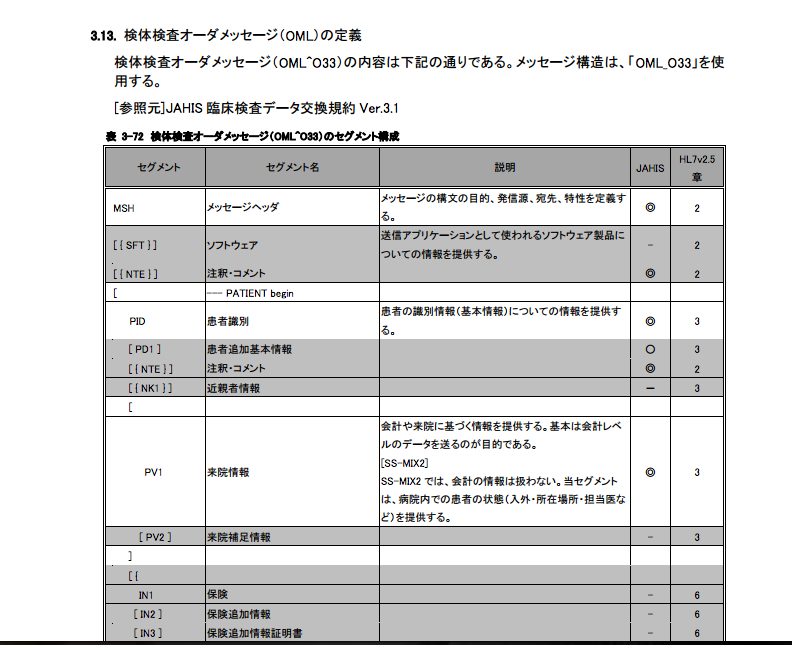
\includegraphics[width=5cm, bb=0 0 645 790]{./gazou/ss-mix_sample.png} %よこたて
		\end{center}
		\caption{データ定義}
		\label{ss-mix_sample}
	\end{figure}

	\begin{figure}[htbp]
		\begin{center}
			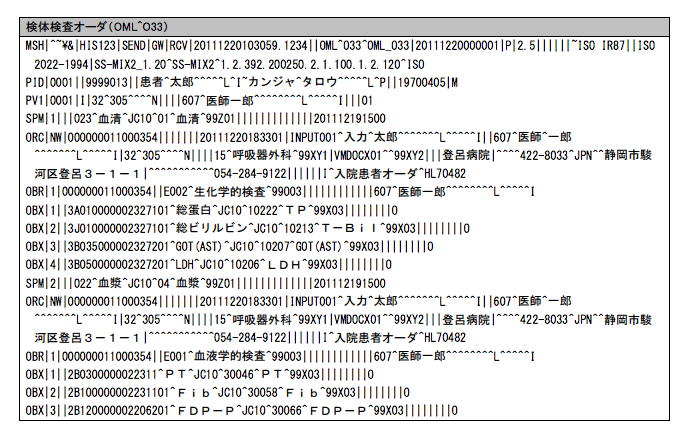
\includegraphics[width=5cm, bb=0 0 437 688]{./gazou/ss-mix_sampledata.png}
		\end{center}
		\caption{データサンプル}
		\label{ss-mix_sampledata}
	\end{figure}

\subsection{アプリケーションの設計}

	\subsubsection{新出のフォーマットのドキュメントに対するコスト}
	縦向き、横向きのcsv(地域の病院で生まれるような電子化された医療情報)はノーコスト.
	電子カルテ固有の出力ファイルはHL7に対応していればノーコスト.
	json型にもってくまでができれば入力できる.
	出力にはkeyを関連付けるためのコストがかかるが,これは利用者がチューニングしていく.

 %医療情報を収集するNoSQLデータベースシステム.UIとしてWebアプリを用意し,
	%医療関係者,薬剤師,患者の3者に対して,情報を扱いやすいようにした.

\subsection{患者情報閲覧}
	ユーザはログイン後,Accountタブから検索ワードを送信すると,
	/getdbでキーに検索ワードを含むヴァリューを表示する.
	ここで,同義のキーで管理されているヴァリューを表示するために
	キー同士の関連が登録されているドキュメントを参照している.



		\begin{figure}[htbp]
				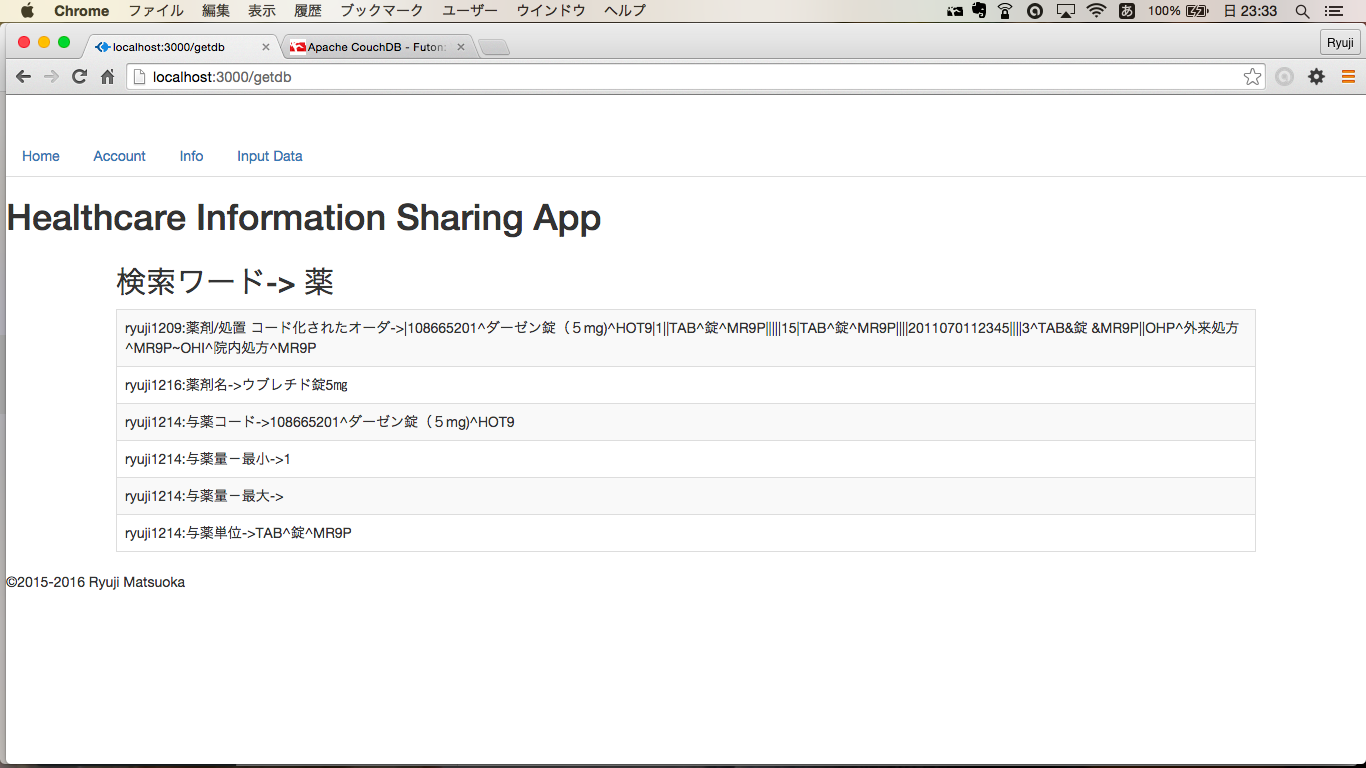
\includegraphics[width=5cm, bb=0 0 437 688]{./gazou/getdb.png}
			\caption{薬 でデータ抽出した様子}
			\label{ss-mix_sampledata}
		\end{figure}



\subsection{データの投入方法}
	ユーザはログイン後,Input Dataタブを選択する.
	次に入力するファイルを選択し,送信する.\ref{fileiopage}

	\begin{figure}[htbp]
		%\begin{center}
			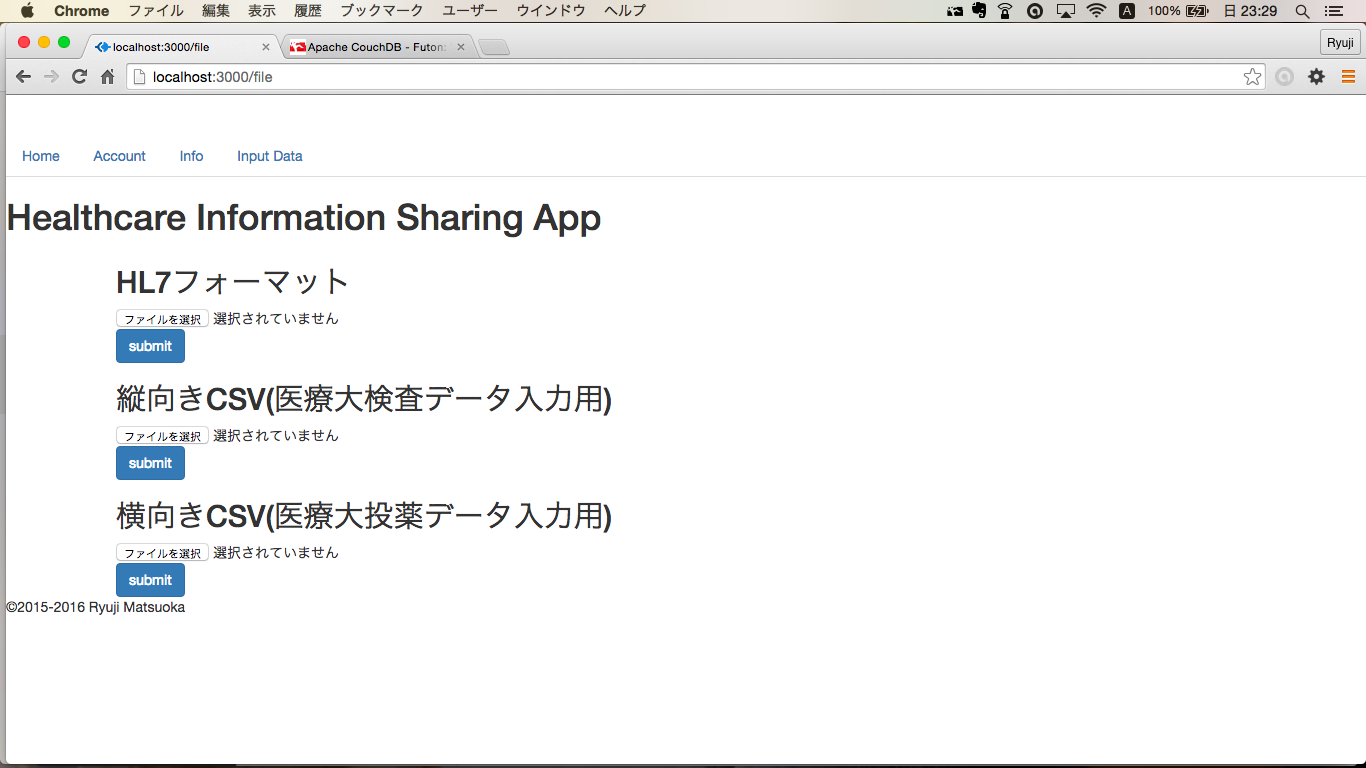
\includegraphics[width=5cm, bb=0 0 437 688]{./gazou/fileiopage.png}
		%\end{center}
		\caption{ファイル入力ページ}
		\label{fileiopage}
	\end{figure}

	1度の診療で1つのドキュメントを生成する.
	CSV入力ファイルに複数回の診療の記録があることを許容する.


	どうやってCouchからデータを引っ張ってきているか.
	患者のドキュメントを検索してからデータを取得.


		\subsubsection{縦向きcsvファイルの場合}
			parse
			医療大の検査データ
			\\
			\begin{figure}[htbp]
				%\begin{center}
					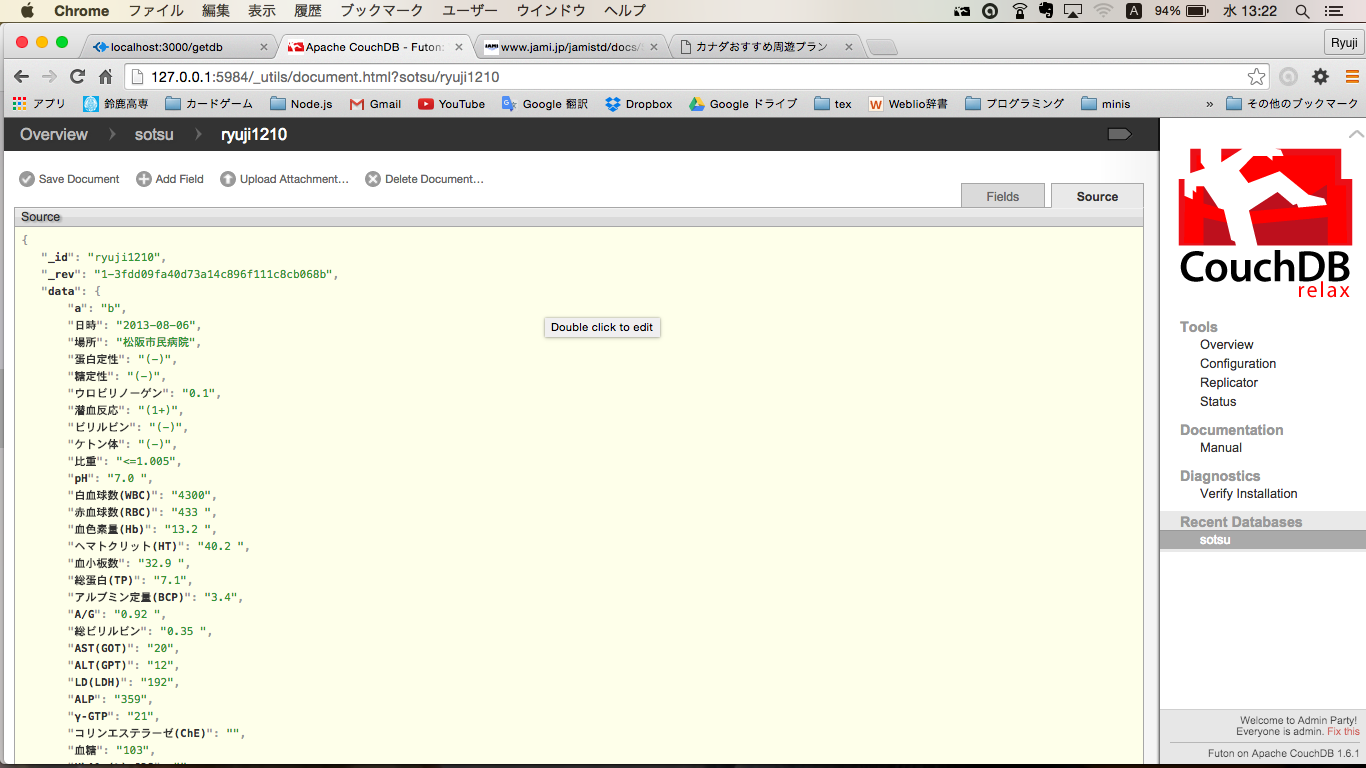
\includegraphics[width=5cm, bb=0 0 437 688]{./gazou/kensa.png}
				%\end{center}
				\caption{医療大の検査データ}
				\label{ss-mix_sampledata}
			\end{figure}

		\subsubsection{横向きcsvファイルの場合}
			holizontialparse
			医療大の投薬データ
			\\
			\begin{figure}[htbp]
				%\begin{center}
					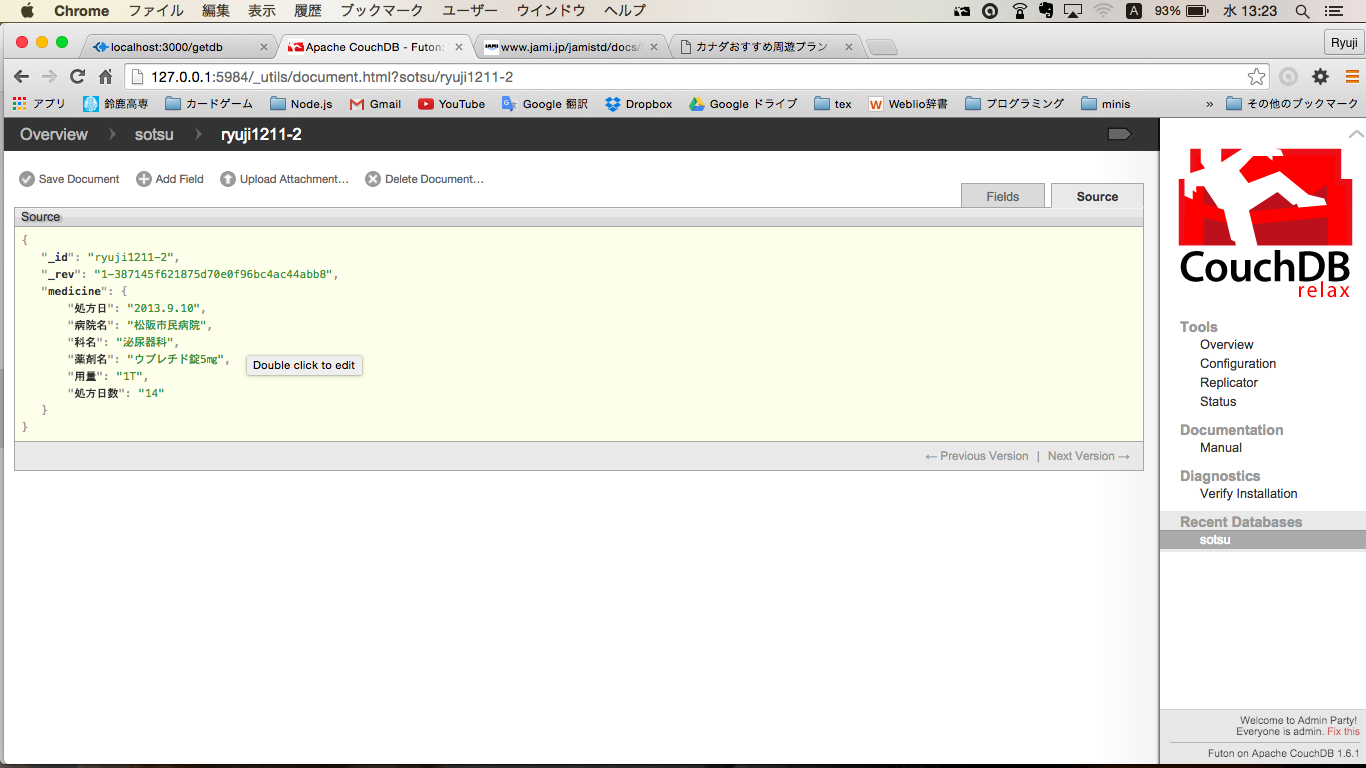
\includegraphics[width=5cm, bb=0 0 437 688]{./gazou/touyaku.png}
				%\end{center}
				\caption{医療大の投薬データ}
				\label{ss-mix_sampledata}
			\end{figure}

		\subsubsection{パイプ区切りのHL7ファイルの場合}
			parsehl7
			HL7のデータ
			\\
			\begin{figure}[htbp]
				%\begin{center}
					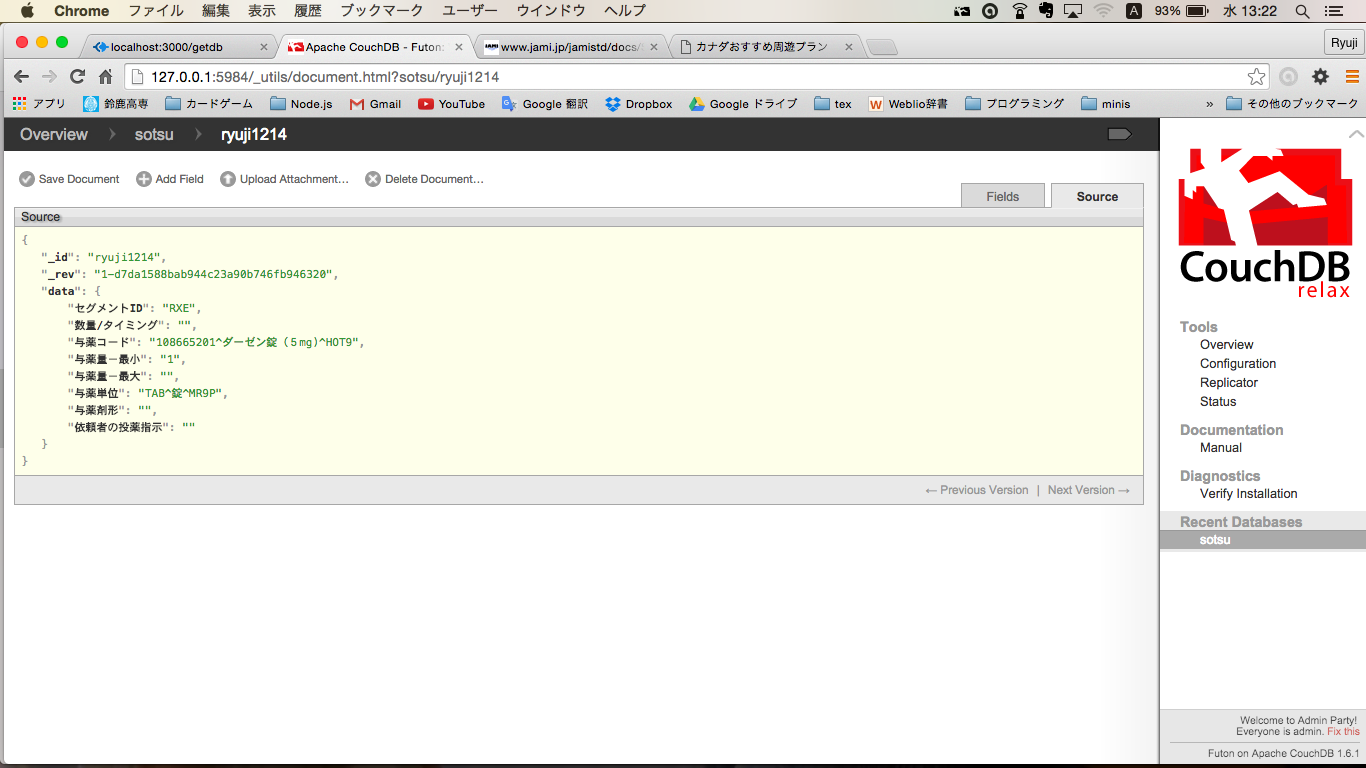
\includegraphics[width=5cm, bb=0 0 437 688]{./gazou/hl7.png}
				%\end{center}
				\caption{HL7のサンプルデータ}
				\label{ss-mix_sampledata}
			\end{figure}



\subsection{同義キーの登録}
	データを参照するときに,キーが必要となる.キーには様々な意味を持つものがあるが,
	異なる規格のデータでは同じ情報を指し示すキーであっても,
	異なるキーが使われている.
	これは新規の規格が医療情報ソフトに流入するたびに課題となる.

	そこで,本研究ではユーザによる同義キーの登録の機能を用意した.
	ユーザは同義である2つのキーを入力すると
	それが同義キーを管理するドキュメントに追加される.

	図\ref{relation}では投薬データの処方日と診断データの日時が同義として登録されている.
	図\ref{relationApp}では検索ワードは処方であるので
	処方をキーに含むデータが検索結果として表示される.
	さらに,検索結果に処方日があり,これは日時と同義として登録されているため,
	日時のデータも検索結果として表示される.
	#実装まだですが.texが嫌になった時にやります。
	#仕様としては、処方日、日時ともにその右に日付がならびます

	\begin{figure}[htbp]
		%\begin{center}
			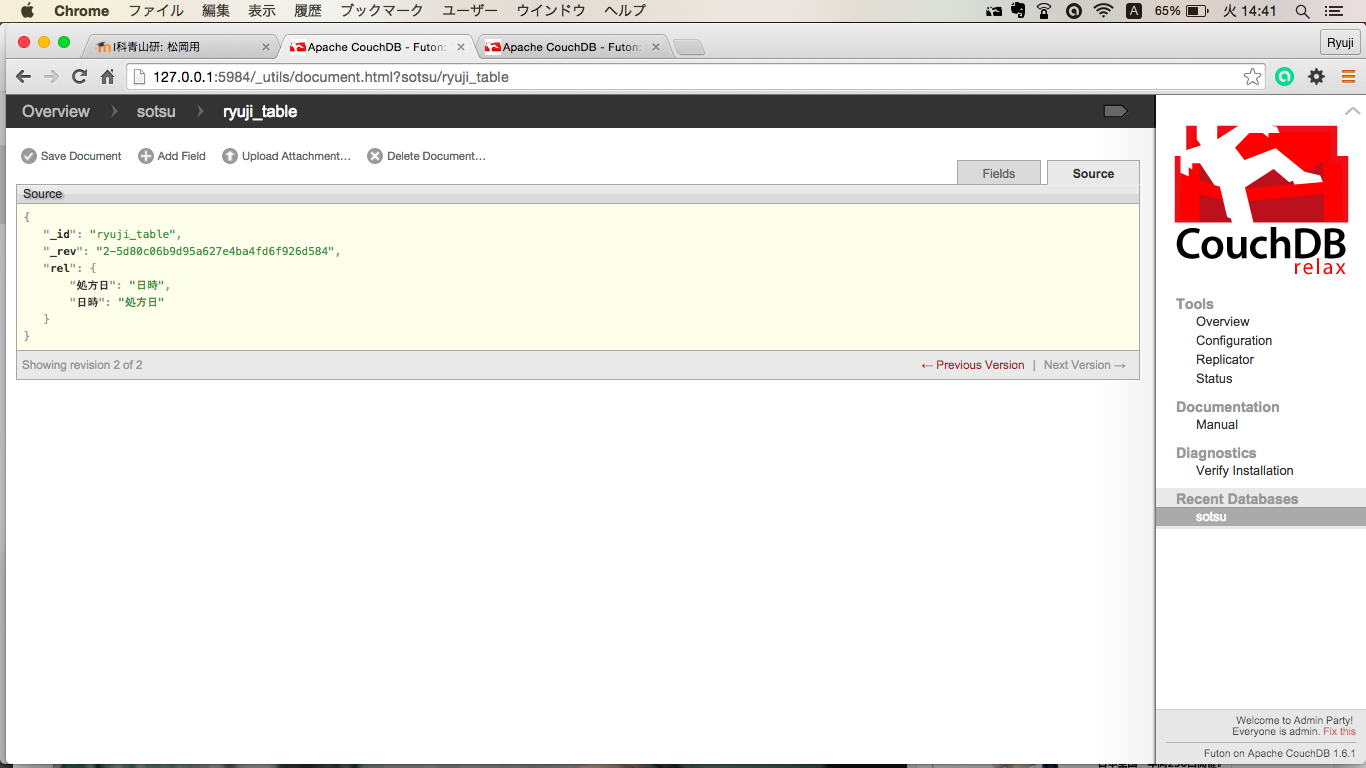
\includegraphics[width=5cm, bb=0 0 437 688]{./gazou/relation.png}
		%\end{center}
		\caption{同義キーを管理するドキュメント}
		\label{relation}
	\end{figure}

	\begin{figure}[htbp]
		%\begin{center}
			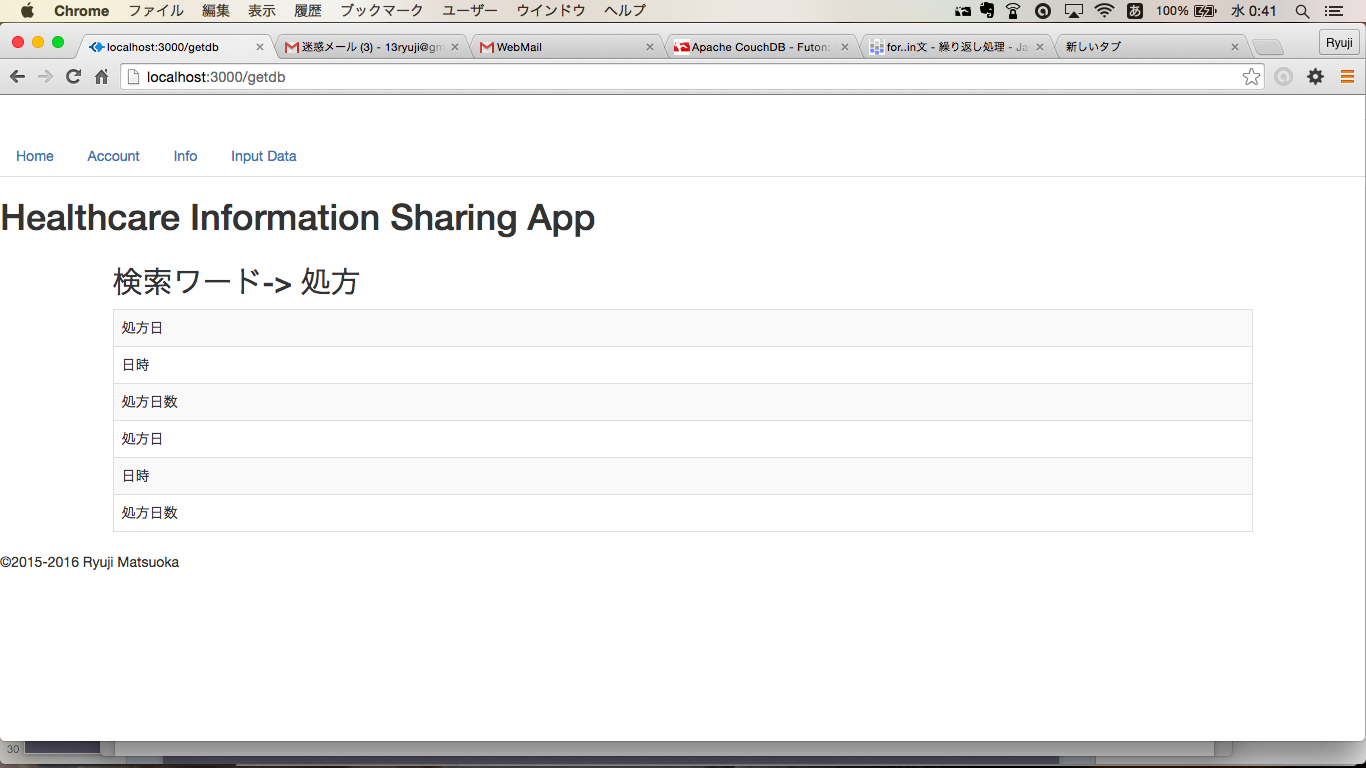
\includegraphics[width=5cm, bb=0 0 437 688]{./gazou/relationApp.png}
		%\end{center}
		\caption{処方と検索して同義キーとして登録されている日時を表示する}
		\label{relationApp}
	\end{figure}
